\chapter{FATファイルシステム}
\label{fatFs}
ファイルシステムの事例としてFATファイルシステムを紹介する.
FATファイルシステムは,
MS-DOS(1981年)からWindows ME(2000年)までで,
OSのシステムディスクに使用された.
それ以降のWindowsではシステムディスク用には使用されていないが,
仕様が公開\footnote{
  \url{http://www.microsoft.com/whdc/system/platform/firmware/fatgen.mspx
  }等から入手できる.}されているので,
USBメモリやメモリカードのファイルシステムとして広く使用されている.

%============================================================================
\section{特徴}
PCだけでなく,様々な電子機器でも用いられ,
広く普及しているファイルシステムである.
Windows,Linux,macOS等もFATファイルシステムをサポートしている.
USBメモリ等を用いて,
異なるオペレーティングシステムや電子機器間でファイルをやり取りできるは,
そのおかげである.
PC以外でも音楽プレーヤ,デジカメ,デジタルテレビ,
カーナビ,電子楽器,計測機器等が,
データの記録やファームウェアのバージョンアップ用にサポートしている.

ファイル名は,半角8文字に加え3文字の拡張子を合わせた最大11文字で表現する.
英字のアルファベットは大文字のみ使用できる.
デジカメの写真データが\|IMG_1234.JPG|\footnote{
  キャノンのデジカメはこのような名前を使用する.}
のようなファイル名になっているのは,
FATファイルシステムの仕様に合わせたためと考えられる.

\tabref{fatVariety}のような,四種類のFATファイルシステムがある.
FAT12,FAT16,FAT32の三つは仕様が無料で入手できるがexFATはそうではない.
また,VFATと呼ばれる規格と合わせて使用すると長いファイル名が使用できる.
以下ではVFATを含まないFAT16の場合を中心に述べる.

\begin{mytable}{btp}{FATファイルシステムの種類}{fatVariety}
  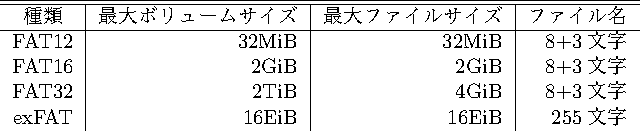
\includegraphics[scale=1.0]{Tbl/fatVariety.pdf}
\end{mytable}

%============================================================================
\section{ボリューム内部の配置}
FATファイルシステムは,
ボリューム(パーティション)内部に\figref{fatVolume}のように配置される.
ここで各領域の意味は次の通りである.

\begin{figure}[btp]
  \centering
  \begin{minipage}{0.4\columnwidth}
    \centering{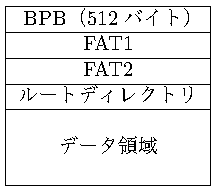
\includegraphics[scale=1.0]{Fig/fatVolume.pdf}}
    \caption{FATボリュームの構造}
    \label{fig:fatVolume}
  \end{minipage}
  \begin{minipage}{0.4\columnwidth}
    \centering{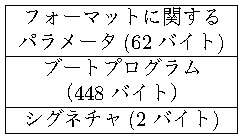
\includegraphics[scale=1.0]{Fig/fatBPB.pdf}}
    \caption{BPB(合計512バイト)}
    \label{fig:bpb}
  \end{minipage}
\end{figure}

\begin{itemize}
\item \emph{BPB(BIOS Parameter Block)}\\
  ボリュームの先頭セクタに配置される.
  内容は\figref{bpb}に示すように,
  FATファイルシステムを初期化する時に決めたパラメータと,
  ブートプログラムである.
  \tabref{fatBpbParam}にBPBに格納される主要な情報を示す.
  この表に掲載した値の例は,
  約2GiBのボリュームをクラスタサイズ32KiBのFAT16フォーマットに
  初期化した例である.
  MBRのブートプログラムはBPBをロードし実行する.
  BPBの先頭には初代PCのCPUである Intel 8086 のJMP機械語命令が置いてあり,
  BPBの後半に格納されたブートプログラムへジャンプする.

\item \emph{FAT(File Allocation Table)}\\
  FATファイルシステムにとって大変重要なデータなので多重化してある.
  FATの数(2重化なら2),
  FATのサイズ(FATあたりのセクタ数)はBPBから知ることができる.

\item \emph{ルートディレクトリ}\\
  FAT領域の直後に固定領域が確保される.
  ルートディレクトリ以外のディレクトリはデータ領域にファイルとして記録される.
  ルートディレクトリサイズはBPBのrootDirサイズに
  エントリ数として記録されている.
  1エントリは32バイトなので,
  \tabref{fatBpbParam}の例では
  ルートディレクトリサイズは$32B \times 512 = 16KiB$になる.
  これをセクタ数に換算すると$16KiB \div 512B = 32セクタ$ になる.

\item \emph{データ領域}\\
  ボリュームの残り領域はファイルの内容データを記録するために使用される.
  データ領域のセクタは\emph{クラスタ}と呼ばれるブロックで扱われる\footnote{
    \tabref{fatBpbParam}の例では1クラスタを64セクタ(32KiB)で構成している.
    この例では1バイトのファイルでも32KiBのデータ領域を
    使用することになりセクタを無駄遣いするが,
    扱えるボリュームサイズを大きくするために,このようになっている.}.
  なお,データ領域に配置されるクラスタの番号は2から始まる.
\end{itemize}

\begin{mytable}{btp}{BPBに格納される主要な情報}{fatBpbParam}
  \centering{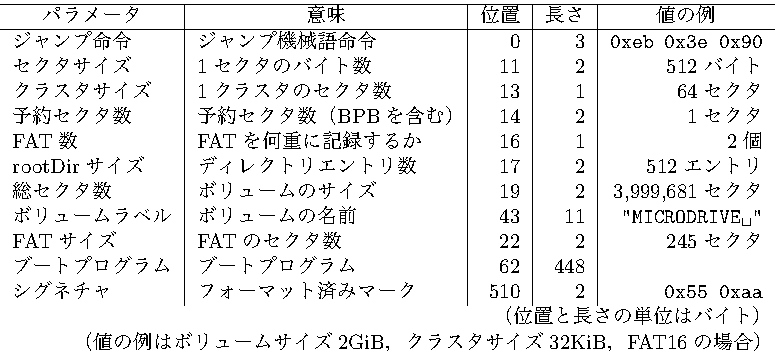
\includegraphics[scale=1.0]{Tbl/fatBpbParameter.pdf}}
\end{mytable}

%============================================================================
\section{ディレクトリエントリ}
ルートディレクトリとディレクトリファイルで共通な
32バイトのデータ構造が使用される.
\figref{fatDirEntry}にディレクトリエントリの構造を図示する.
各部の意味は次の通りである.

\begin{myfig}{btp}{ディレクトリエントリ}{fatDirEntry}
  \centering{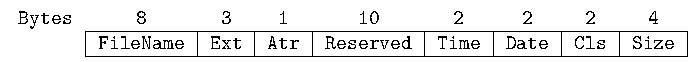
\includegraphics[scale=1.0]{Fig/fatDirEntry.pdf}}
\end{myfig}

\begin{itemize}
\item \|FileName|は8文字以内のファイル名である.\\
  左づめで格納し,余ったバイトはスペース(\|0x20|)で埋める.
  \|FileName|の第一バイトが
  \|0x00|の場合は,
  そのエントリーと以降のエントリーが使用されていないことを表す\footnote{
    ディレクトリファイルのEOFを表現している.}.
  \|0xe5|の場合は,エントリーが削除されていることを表す.
  \|0x05|の場合は,本来の第一バイトが文字コード\|0xe5|であることを表す.
  リスト\ref{tacosReadFname}にTacOSのソースプログラム\footnote{
    \url{https://github.com/tctsigemura/TacOS/blob/master/os/fs/dirAccess.cmm}
  }中で,エントリからファイル名を読む部分を示す.
  文字コード\|0x05|の扱いを確認してほしい.

\item \|Ext|は3文字以内のファイル名の拡張子である.

\item \|Atr|にはファイルの属性を格納する.\\
  read-only(\|0x01|),hidden(\|0x02|),
  system-file(\|0x04|),archive(\|0x20|),
  directory(\|0x10|)等の属性がある.
  directoryはそのファイルがディレクトリファイルであることを,
  archiveは前回のバックアップ後にファイルが変更されたことを表す.
  ビットを組合せて属性を表現する.
  例えば\|0x03|は,読み出し専用の隠しファイルの意味になる.

\item \|Reserved|は未使用の領域である.

\item \|Time|はファイルの最終変更時刻を2秒の精度で表現する\footnote{
  下位ビットから順に,$秒 \div 2$(5ビットなので2秒単位),
  分(6ビット),
  時(5ビット)で表現する.}.

\item \|Date|はファイルの最終変更日を表現する\footnote{下位ビットから順に,
  日(5ビット),月(4ビット),$年-1980$(7ビット)で表現する.
  2108年問題を含んでいる.}.

\item \|Cls|はファイルのデータが格納されている\emph{先頭クラスタの番号}である.
  
\item \|Size|はバイト単位で表したファイルのサイズである.
  ディレクトリファイルの場合は 0 にする.
\end{itemize}

\lstinputlisting[float=btp,caption=ファイル名を読み出すプログラム,
  firstline=86,lastline=94,
  numbers=none,label=tacosReadFname]{TacOS/fs/dirAccess.cmm}

%============================================================================
\section{FAT(File Allocation Table)}
FATは,\figref{fatConcept}のような表である.
\figref{fatFileSystem}のように,
FATのエントリとデータ領域のクラスタが,一対一に対応する.
エントリには,ファイル中で次のクラスタの番号を格納する.
同一ファイルのデータ領域は,
FAT中に表現されたクラスタのチェインにより辿ることができる.
エントリが12ビットの場合をFAT12,
16ビットの場合をFAT16,28ビットの場合をFAT32と呼ぶ.
以下では\emph{FAT16の場合}を例に説明する.

\begin{itemize}
\item \emph{エントリ値の意味} \\
  FATエントリに書き込まれる値の意味を\tabref{fatClsNum}にまとめる.
  \|0x0000|は,そのエントリが使用されていないことを表す.
  \|0x0001|は,何かの意味を割当てるために予約されている\footnote{
    TacOSの内部処理では,ルートディレクトリのクラスタ番号として利用している.
  }.\|0x0002|〜\|0xfff6|が普通のクラスタ番号である.
  よって,最大65,525個\footnote{
    $0xFFF6 - 1 = 0xFFF5 = 65,525$
  }のクラスタに番号を付けることができる.
  \|0xfff7|は不良クラスタ\footnote{
    何かの理由で正しく読み書きできないセクタが含まれるクラスタのこと.
  }を表す.
  \|0xfff8|〜\|0xffff|は,
  クラスタチェインの終わり(ファイルの終わり)を表している.
  FATエントリの\|0x0000|が未使用クラスタ(空きクラスタ)を表すので,
  FATは空き領域管理の役割も担っている.

\item \emph{クラスタチェイン} \\
  FATエントリに\emph{次クラスタの番号}を書き込むことにより,
  \emph{クラスタチェイン}を作る.
  例えば\figref{fatConcept}は,
  第2,第4,第5クラスタからなるチェインを含んでいる.
  第5クラスタの\|0xffff|はチェインの終わりを表している.
  一つのチェインがファイルに属するクラスタのリストを表現している.
  チェインの先頭(ファイルの先頭)はディレクトリエントリの\|Cls|から分かる.

  FATファイルシステムはクラスタチェインを作るので,
  データブロックを\emph{リンク方式}で管理していると言える.
  FATを順に調べることでランダムアクセスができるが,
  \emph{順に}調べる必要がある.

\end{itemize}

\begin{table}[btp]
  \centering
  \begin{minipage}[c]{0.4\textwidth}
    \makeatletter
    \def\@captype{figure}
    \makeatother
    \centerline{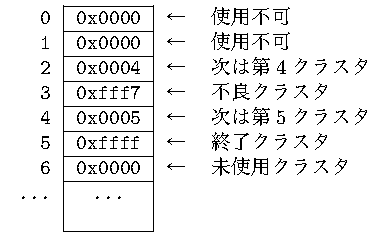
\includegraphics[scale=1.0]{Fig/fatConcept.pdf}}
    \caption{FATの仕組み}
    \label{fig:fatConcept}
  \end{minipage}
  \begin{minipage}{0.5\textwidth}
    \caption{FATエントリ値の意味}
    \label{tab:fatClsNum}
    \centerline{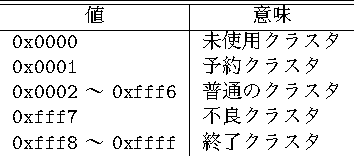
\includegraphics[scale=1.0]{Tbl/fatClsNum.pdf}}
  \end{minipage}
\end{table}

%============================================================================
\section{ディレクトリファイル}
ルートディレクトリ以外の(サブ)ディレクトリは,
\|Atr|のdirectory(0x10)属性がONになったファイルである.
これを\emph{ディレクトリファイル}と呼ぶ.
ディレクトリファイルにはルートディレクトリと
同じ形式のディレクトリエントリを記録する.
ディレクトリファイルもクラスタチェインでデータ領域を割り付けられるので,
\tabref{fatBpbParam}の構成なら最低でも32KiBの大きさになる.

リスト\ref{fatDirDump}に,
macOSでFAT16ファイルシステム上にディレクトリ\|A|を作成し,
ディレクトリファイル\|A|を16進ダンプした例を示す.
\|00000080|以降は全てのデータが\|00|なので\|*|が表示され省略されているが,
最後の行の\|00008000|からファイルサイズが32KiBであることが分かる.
また,\|00000000|からカレントディレクトリ「\|.|」を表すエントリ,
\|00000020|から親ディレクトリ「\|..|」を表すエントリが格納されている.
\|00000040|からディレクトリ\|DIR|を表すエントリ,
\|00000060|からファイル\|A.TXT|を表すエントリが格納されている.
\figref{fatDirEntry}と比較しながら解析して欲しい.

\lstinputlisting[float=btp,
  caption=FATファイルシステムのディレクトリの16進ダンプ結果,
  numbers=none,label=fatDirDump]{Lst/fatDirDump.txt}

%============================================================================
\section{FATファイルシステムの全体像を示す例}
\tabref{fatBpbParam}に例示したパラメータで初期化されたFATファイルシステムに
65KiBの\|\ABCDEFGH.TXT|と,
1KiBの\|\SAMPLE.DAT|の二つのファイルが書き込まれた状態を
\figref{fatFileSystem}に示す.

\begin{myfig}{bp}{FATファイルシステムにファイルを格納した例}{fatFileSystem}
  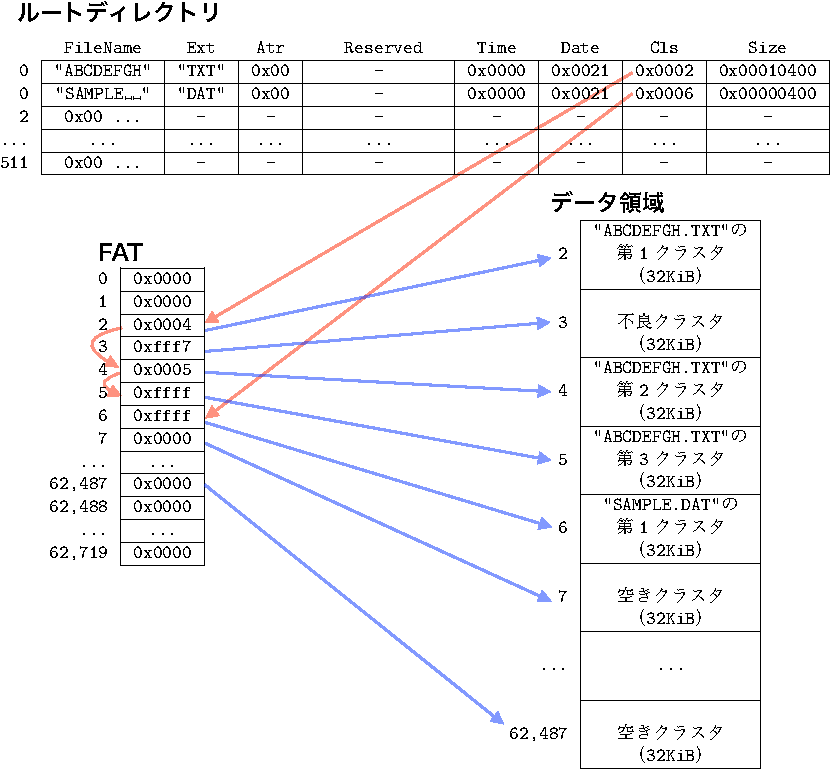
\includegraphics[scale=1.0]{Fig/fatFileSystem-crop.pdf}
\end{myfig}

\begin{itemize}
\item \emph{ルートディレクトリ}\\
  \tabref{fatBpbParam}の例ではルートディレクトリは512エントリからなり,
  32セクタ使用することになっている.
  リスト\ref{fatDirDump}ではカレントディレクトリ「\|.|」と
  親ディレクトリ「\|..|」が格納されていたが,
  ルートディレクトリには存在しない.
  \figref{fatFileSystem}では,
  先頭の2エントリを用い2つのファイルが登録されている.
  通常ファイルなので\|Atr|は\|0x00|である.
  最終変更日時は1980年1月1日0時を表す値になっている.
  \|Cls|に格納された値がFAT上のクラスタチェイン開始エントリを指している.
  \|Size|は65KiBを表す\|0x00010400|と1KiBを表す\|0x00000400|になっている.
  3つ目のエントリ以降は使用されていないので\|FileName|の第1バイトが
  空きを意味する\|0x00|になっている.

\item \emph{FAT}\\
  \tabref{fatBpbParam}の例では,FATは245セクタ使用することになっている.
  セクタサイズが512バイト,FATエントリは16ビット(2バイト)なので
  1セクタに256エントリ格納できる.
  FAT全体のエントリ数は
  $245 \times 256 = 62,720$になり,
  FATのエントリ番号は0から62,719の範囲である.

  ルートディレクトリの\|ABCDEFGH.TXT|エントリから,
  このファイルは第2クラスタから始まるクラスタチェインに格納されることが分かる.
  FATの内容を確認すると
  第2,第4,第5クラスタからなる長さ3のチェインになっているので,
  \|ABCDEFGH.TXT|ファイルのデータは,これら3クラスタを使用して格納される.
  3クラスタの合計容量は96KiBなので65KiBのファイルを
  格納するには十分である\footnote{2クラスタでは64KiBまでしか格納できない.}.

  ルートディレクトリの\|SAMPLE.DAT|エントリから,
  このファイルは第6クラスタから始まるクラスタチェインに格納されることが分かる.
  FATの内容を確認すると
  第6クラスタがチェインの最終クラスタなのでチェインの長さは1である.
  \|SAMPLE.DAT|ファイルのデータは第6クラスタに格納される.

\item \emph{データ領域}\\
  \tabref{fatBpbParam}の例では,ボリューム全体で3,999,681セクタである.
  BPB(1セクタ),FAT1(245セクタ),FAT2(245セクタ),
  ルートディレクトリ(32セクタ)であるので,
  残り$3,999,681 - 1 - 245 \times 2 - 32 = 3,999,158$セクタが
  データ領域として使用できる.

  クラスタサイズは64セクタなので,データ領域は
  $3,999,158 \div 64 = 62,486$クラスタ(余り54セクタ\footnote{
      余り54セクタは使用できない.
  })になる.
  データ用クラスタの番号は2番から始めることになっている
  (\tabref{fatClsNum}参照)ので,
  2番から62,487番までがデータ領域のクラスタ番号になる.
  FATエントリは62,719番まで用意されているが,
  62,488番から62,719番は使用されない.

  \|ABCDEFGH.TXT|ファイルのクラスタチェインは,
  第2,第4,第5クラスタなので,
  ファイルデータが先頭から32KiBずつ第2,第4クラスタに置かれる.
  第5クラスタは,先頭にファイル末尾の1KiBが置かれ残り31KiBは使用されない.
\end{itemize}

%============================================================================
\section{実装例}
第\ref{tacosFAT}章にTacOSのファイルシステムサーバ(fs)の実装例を示す.
この実装例は,
FAT16専用のファイルシステム管理プログラムを{\cmml}で記述したものである.

%============================================================================
\section{まとめ}
FATファイルシステムは,
USBメモリやメモリカードで使用されている.
多くのオペレーティングシステムや電子機器が
FATファイルシステムをサポートしているので,
オペレーティングシステムや機器の種類を越えて
データを交換するために盛んに使用されている.

この章では特にFAT16ファイルシステムについてかなり踏み込んだ解説を行った.
ボーリューム内部の配置,ディレクトリエントリ,FAT,
ディレクトリファイルを具体的な値を示しながら説明した.
また,第\ref{tacosFAT}章にはTacOSのFAT16ファイルシステムサーバの
実装例を掲載している.

%==============================================================================
\section*{練習問題}
\begin{enumerate}
  \renewcommand{\labelenumi}{\ttfamily\arabic{chapter}.\arabic{enumi}}
  \setlength{\leftskip}{1em}
\item 次の言葉の意味を説明しなさい.
  \begin{enumerate}
  \item BPB
  \item ルートディレクトリ
  \item クラスタ
  \item ディレクトリエントリ
  \item FAT
  \item クラスタチェイン
  \item ディレクトリファイル
  \end{enumerate}
\item リスト\ref{fatDirDump}を
  \figref{fatDirEntry}と比較しながら解析しなさい.
\item \figref{fatFileSystem}の\|ABCDEFGH.TXT|ファイルの
  第\|0x00002000|バイトが格納されるクラスタの番号を答えなさい.
\item 前問と同様に,
  第\|0x00004000|,\|0x00008000|,\|0x00010000|
  バイトに付いて答えなさい.
\end{enumerate}
